\documentclass[man,floatsintext]{apa6}
\usepackage{lmodern}
\usepackage{amssymb,amsmath}
\usepackage{ifxetex,ifluatex}
\usepackage{fixltx2e} % provides \textsubscript
\ifnum 0\ifxetex 1\fi\ifluatex 1\fi=0 % if pdftex
  \usepackage[T1]{fontenc}
  \usepackage[utf8]{inputenc}
\else % if luatex or xelatex
  \ifxetex
    \usepackage{mathspec}
  \else
    \usepackage{fontspec}
  \fi
  \defaultfontfeatures{Ligatures=TeX,Scale=MatchLowercase}
\fi
% use upquote if available, for straight quotes in verbatim environments
\IfFileExists{upquote.sty}{\usepackage{upquote}}{}
% use microtype if available
\IfFileExists{microtype.sty}{%
\usepackage{microtype}
\UseMicrotypeSet[protrusion]{basicmath} % disable protrusion for tt fonts
}{}
\usepackage{hyperref}
\hypersetup{unicode=true,
            pdftitle={Does Your Gain Define My Loss?: Socially-Defined Counterfactual Loss and Prevention-Focused Decision-Making},
            pdfauthor={{[}Anonymous Author(s){]}},
            pdfkeywords={motivation, self-regulation, regulatory focus, prevention, decision-making, risk, counterfactual thinking},
            pdfborder={0 0 0},
            breaklinks=true}
\urlstyle{same}  % don't use monospace font for urls
\usepackage{graphicx}
% grffile has become a legacy package: https://ctan.org/pkg/grffile
\IfFileExists{grffile.sty}{%
\usepackage{grffile}
}{}
\makeatletter
\def\maxwidth{\ifdim\Gin@nat@width>\linewidth\linewidth\else\Gin@nat@width\fi}
\def\maxheight{\ifdim\Gin@nat@height>\textheight\textheight\else\Gin@nat@height\fi}
\makeatother
% Scale images if necessary, so that they will not overflow the page
% margins by default, and it is still possible to overwrite the defaults
% using explicit options in \includegraphics[width, height, ...]{}
\setkeys{Gin}{width=\maxwidth,height=\maxheight,keepaspectratio}
\IfFileExists{parskip.sty}{%
\usepackage{parskip}
}{% else
\setlength{\parindent}{0pt}
\setlength{\parskip}{6pt plus 2pt minus 1pt}
}
\setlength{\emergencystretch}{3em}  % prevent overfull lines
\providecommand{\tightlist}{%
  \setlength{\itemsep}{0pt}\setlength{\parskip}{0pt}}
\setcounter{secnumdepth}{0}
% Redefines (sub)paragraphs to behave more like sections
\ifx\paragraph\undefined\else
\let\oldparagraph\paragraph
\renewcommand{\paragraph}[1]{\oldparagraph{#1}\mbox{}}
\fi
\ifx\subparagraph\undefined\else
\let\oldsubparagraph\subparagraph
\renewcommand{\subparagraph}[1]{\oldsubparagraph{#1}\mbox{}}
\fi

%%% Use protect on footnotes to avoid problems with footnotes in titles
\let\rmarkdownfootnote\footnote%
\def\footnote{\protect\rmarkdownfootnote}


  \title{Does Your Gain Define My Loss?: Socially-Defined Counterfactual Loss and Prevention-Focused Decision-Making}
    \author{{[}Anonymous Author(s){]}\textsuperscript{a}}
    \date{}
  
\shorttitle{Social Counterfactual Loss and Prevention Focus}
\affiliation{
\vspace{0.5cm}
\textsuperscript{a} [Anonymized Institution(s)]}
\keywords{motivation, self-regulation, regulatory focus, prevention, decision-making, risk, counterfactual thinking\newline\indent Word count: 4,967}
\usepackage{csquotes}
\usepackage{upgreek}
\captionsetup{font=singlespacing,justification=justified}

\usepackage{longtable}
\usepackage{lscape}
\usepackage{multirow}
\usepackage{tabularx}
\usepackage[flushleft]{threeparttable}
\usepackage{threeparttablex}

\newenvironment{lltable}{\begin{landscape}\begin{center}\begin{ThreePartTable}}{\end{ThreePartTable}\end{center}\end{landscape}}

\makeatletter
\newcommand\LastLTentrywidth{1em}
\newlength\longtablewidth
\setlength{\longtablewidth}{1in}
\newcommand{\getlongtablewidth}{\begingroup \ifcsname LT@\roman{LT@tables}\endcsname \global\longtablewidth=0pt \renewcommand{\LT@entry}[2]{\global\advance\longtablewidth by ##2\relax\gdef\LastLTentrywidth{##2}}\@nameuse{LT@\roman{LT@tables}} \fi \endgroup}
\usepackage{setspace}
\usepackage{makecell}
\raggedbottom

\authornote{a {[}Anonymized Corresponding Author Address(es){]}

Declarations of interest: none

This research did not receive any specific grant from funding agencies in the public, commercial, or not-for-profit sectors.

Correspondence concerning this article should be addressed to {[}Anonymous Author(s){]}, {[}Anonymized Corresponding Author Address{]}. E-mail: {[}Anonymized Author Email{]}}

\abstract{
How do individual differences in motivation relate to risky decision-making? This article focuses on cases of a socially-defined counterfactual loss---situations in which the people in one's social context experience a gain, and this successful state functions as a new ``status quo'' reference point against which the individual falls short. Although a prevention focus is known to predict risky investment behavior following \emph{actual} loss (Scholer, Zou, Fujita, Stroessner, \& Higgins, 2010), there is as yet no research exploring whether a prevention focus similarly predicts risk-taking after this kind of \emph{counterfactual} loss. The objective of the present study was to explore this relation within a real-world situation in which participants invested in Bitcoin, a risky asset. Results revealed that stronger chronic prevention focus predicted decreased risk-taking among participants who experienced a counterfactual loss; no such effect was detected among a control group (to dynamically visualize model-predicted effects, see \url{http://regfocusrisk.com}). Further, this effect was mediated by hypothetical feelings of relief when imagining that one had previously invested in Bitcoin. This research extends previous findings on the relationship between regulatory focus and risk-seeking, and offers implications for everyday decision-making. Data and syntax can be found at \url{https://osf.io/e4nr3/?view_only=73c8490e19c6449197d2620d29ea8ad2} {[}de-anonymized URL provided following peer review{]}.


}

\begin{document}
\maketitle

\hypertarget{introduction}{%
\section{1. Introduction}\label{introduction}}

How do people determine how their goal pursuits are going? A large body of research suggests that reference points play a critical role in this process (e.g., Bonezzi, Brendl, \& De Angelis, 2011; Heath, Larrick, \& Wu, 1999). These reference points function as self-evaluative standards (Higgins, Strauman, \& Klein, 1986) and influence whether a person decides to take or avoid a risk (Higgins \& Liberman, 2018). Although these reference points are often rooted in \emph{personal} standards, they can also be defined by the \emph{social} context (Higgins et al., 1986). Consider a case in which the value of the risky cryptocurrency Bitcoin spikes. Upon hearing that friends profited from this increase, people with no investments in Bitcoin may be upset not to have obtained these same benefits. In this case, while these investors have not actually lost anything, their peers have set a new status quo below which they fall---a situation we define as a \emph{counterfactual loss}.

But what predicts how a given investor will respond to such a situation? Some people might engage in risky behavior (e.g., investing a large sum in Bitcoin) in an attempt to reach this new status quo. In contrast, others may recommit themselves to a risk-averse investing strategy. To answer this question, we investigated whether individual differences that influence responses to \emph{actual} loss might similarly predict responses to \emph{counterfactual} loss.

One such individual difference variable is a prevention focus. The prevention system is strategically oriented toward the avoidance of actual loss as it is motivated by fundamental needs for safety and security (Higgins, 1997). A prevention focus is also known to influence one's tendency to make risky choices: Although generally risk-averse in the investment domain (Zou \& Scholer, 2016), people high in prevention tend to take greater risks after incurring a loss in an effort to bring themselves back to baseline (Scholer et al., 2010).

This kind of loss is different from \emph{counterfactual} loss because counterfactual loss does not actually threaten individuals' safety. However, given the high relevance of actual loss states to prevention-focused people, we were curious if they would respond to counterfactual losses in a similar way. As a result, the purpose of the present study was to investigate the relationship between regulatory focus and risky decision-making following counterfactual loss within an ecologically-valid investing paradigm. This work is important because risky choices may result in undesirable consequences, and follow-up research might reveal how individuals could mitigate these tendencies.

\hypertarget{regulatory-focus-theory}{%
\subsection{1.1. Regulatory Focus Theory}\label{regulatory-focus-theory}}

Regulatory focus theory posits two distinct motivational orientations that vary based upon the end-states at which self-regulatory efforts are directed: A \emph{prevention} focus involves strategic concerns with \emph{negative} outcomes like losses, whereas a \emph{promotion} focus reflects strategic concerns with \emph{positive} outcomes like gains (Higgins, 1997). Prevention-focused people are interested in maintaining a satisfactory status quo (\enquote{0}) and avoiding worse states (\enquote{--1}); in contrast, promotion-focused people are interested in moving from their status quo (\enquote{0}) to a better state (``+1''; Higgins, 2018). These individual difference variables predict unique patterns of goal-directed thinking and behavior (see Higgins \& Cornwell, 2016, for a review).

\hypertarget{regulatory-focus-and-risky-decision-making.}{%
\subsubsection{1.1.1. Regulatory focus and risky decision-making.}\label{regulatory-focus-and-risky-decision-making.}}

Prevention and promotion are also associated with distinct risk-seeking tendencies. As briefly described above, prevention predicts risk-taking in the face of loss (Scholer et al., 2010). In these studies, after experiencing an initial financial loss, participants chose between two stocks with explicitly-stated odds---both of which offered the same expected value but different levels of risk. Results suggested that a prevention focus predicted selection of the riskier stock in cases when this option provided the only chance of recouping previous losses and returning to the status quo. However, when a less risky option offered this same possibility, prevention was associated with risk aversion. (Similar associations exist between promotion and risk-seeking in cases of recent gains; see Zou, Scholer, \& Higgins, 2014.)

Because actual and counterfactual loss may produce similar internal experiences, we expected that the prevention system might operate similarly in both cases. As a result, we primarily hypothesized that a prevention focus will predict \emph{greater} risky behavior following counterfactual loss, such that people high in prevention will take larger risks in attempting to recover the \enquote{lost} amount when the risky action offers the sole chance to attain the new socially-determined satisfactory state. In the present research, we intended to provide such an opportunity through the ability to invest in Bitcoin.

However, an alternate account is also feasible. As described above, in cases when no option exists to \emph{fully} recover a loss, prevention is associated with risk aversion (Scholer et al., 2010). If participants do not believe that the risky asset offers the opportunity to fully recover the counterfactual loss, we would predict the reverse effect, whereby participants high in prevention will engage in \emph{less} risky behavior in the case of counterfactual loss.

\hypertarget{regulatory-focus-and-emotion.}{%
\subsubsection{1.1.2. Regulatory focus and emotion.}\label{regulatory-focus-and-emotion.}}

Emotions relating to the counterfactual situation may provide insight into the underlying mechanism because emotional experiences vary based upon regulatory focus. In the domain of prevention, success is typically associated with quiescence-related emotions (e.g., relief), while failure is accompanied by agitation-related emotions (e.g., nervousness; Higgins, 1996). Further, experiences on this quiescence-agitation spectrum increase in frequency and intensity with prevention strength (Higgins et al., 1997).

To investigate these emotional experiences, we asked participants to imagine how they would feel if they had invested in Bitcoin earlier. Given our interest in prevention, we were especially interested in hypothetical \emph{relief}, which we expect would be rooted in imagined anxiety about what might have happened differently. As a result, participants' willingness to actually experience that level of anxiety by making a risky investment today may be mediated by this hypothetical relief. With this said, we did not pre-register any hypotheses regarding mediation; these analyses were exploratory.

\hypertarget{methods}{%
\section{2. Methods}\label{methods}}

\hypertarget{participants}{%
\subsection{2.1. Participants}\label{participants}}

A pilot study examining the interaction between prevention and risk-taking in cases of counterfactual loss suggested an \(f^2\) effect size of 0.021. A power analysis suggested a sample size of 462; to account for attrition, we enrolled 500 participants. (See \url{https://osf.io/e4nr3/?view_only=73c8490e19c6449197d2620d29ea8ad2} for pre-registered sample size, analysis plans, data, and syntax {[}de-anonymized URL to be provided following blind peer review{]}.)

Data collection took place in September 2018. Using Amazon Mechanical Turk (\enquote{M-Turk}), we recruited U.S. workers at least 18 years old. Per our pre-defined exclusion criteria, 19 participants were excluded for not completing our primary measures. Additionally, 180 participants were excluded for fraudulent IP addresses.\footnote{At the time of this study, data quality issues had recently surfaced on M-Turk due to foreign workers' use of Virtual Private Servers (see, for example, Kennedy et al., 2018). As a result, we examined our dataset for fraudulent responses based on participant IP addresses using using the R-package \emph{rIP} (Version 0.1.1; Kennedy \& Waggoner, 2018). (See Supplementary Materials for more detail on this investigation.) Due to significant reliability issues among the responses flagged as fraudulent, we excluded these participants.} Finally, we excluded 6 participants who learned about the study from other M-Turk workers (although all analyses were also run including this last group to ensure key findings did not change). These exclusions left a sample of 295 participants (\(M_{age} = 36.43\); 50.17\% male).

\hypertarget{material}{%
\subsection{2.2. Material}\label{material}}

\hypertarget{regulatory-focus-pride.}{%
\subsubsection{2.2.1. Regulatory focus pride.}\label{regulatory-focus-pride.}}

To measure chronic historical effectiveness (i.e., \enquote{pride}) in the domains of prevention and promotion, we administered the Regulatory Focus Questionnaire (``RFQ''; Higgins et al., 2001). The RFQ consists of five prevention-related items (e.g., \enquote{Not being careful enough has gotten me into trouble at times}) and six promotion-related items (e.g., \enquote{I feel like I have made progress toward being successful in my life}) to which participants respond on five-point scales ranging from 1 (\emph{never or seldom} or \emph{certainly false}) to 5 (\emph{very often} or \emph{certainly true}). Mean endorsement levels were calculated for each participant (\(M_{prevention} = 3.44\); \(SD_{prevention} = 0.89\); \(\alpha_{prevention} = 0.88\); \(M_{promotion} = 3.44\); \(SD_{promotion} = 0.69\); \(\alpha_{promotion} = 0.73\)). We then centered these variables by subtracting these means from each score.

\hypertarget{counterfactual-loss-manipulation.}{%
\subsubsection{2.2.2. Counterfactual loss manipulation.}\label{counterfactual-loss-manipulation.}}

Participants were randomly assigned to one of two experimental conditions: counterfactual loss versus control. After an introduction to an investing app that they would beta-test, participants in the counterfactual loss condition were notified that they were joining a test-in-progress on Day 4, while participants in the control condition were simply welcomed to Day 1 of the beta-test:

\begin{quote}
\textbf{{[}Counterfactual Loss:{]}} Please note that you will be joining on Day 4, as we expanded the testing group midway through the beta-test in order to receive feedback from a larger group of participants. Despite any earnings or losses that the original group of M-Turk participants may have incurred since Day 1, you will be starting today with your \$1 bonus---as if this \$1 was kept in savings (i.e., with 0\% invested in Bitcoin) over the last three days.
\end{quote}

\begin{quote}
\textbf{{[}Control:{]}} We welcome you and your fellow participants to Day 1 of our beta-test!
\end{quote}

Next, all participants learned that Bitcoin had risen in price over the previous three days. This information was framed differently in each condition. Participants in the counterfactual loss condition were told that fellow M-Turk participants who joined the testing group at an earlier date and invested at 100\% had already increased the value of their own \$1 investments to \$1.61; in contrast, participants in the control condition who believed they were joining the test on Day 1 learned that \$1 would have \emph{hypothetically} grown to \$1.61 during the same timeframe (see Figure~\ref{fig:manip}). Additionally, to reinforce that their present state fell below the reference point set by their M-Turk peers, participants in the counterfactual loss condition also saw a flat line indicating their current status.

\begin{figure}

{\centering 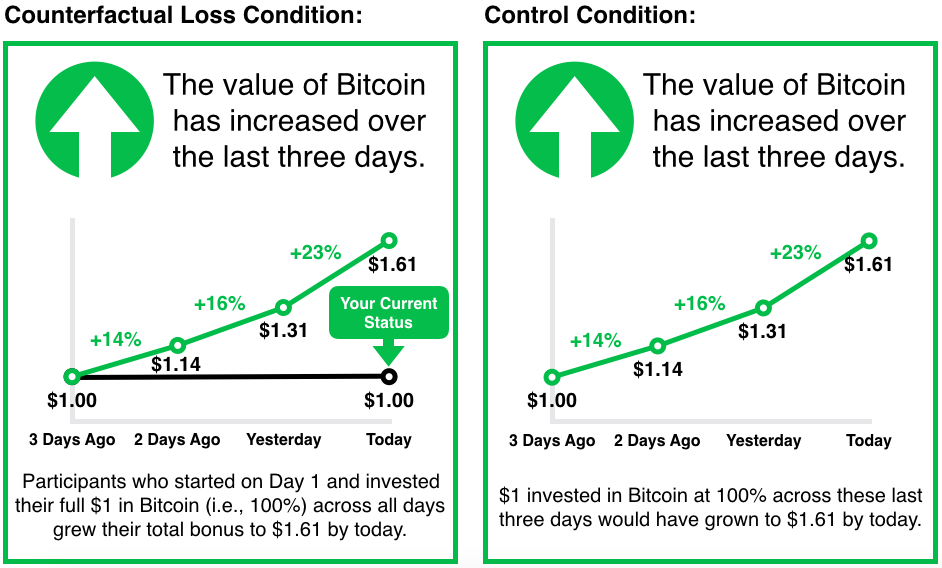
\includegraphics[width=0.9\linewidth,height=0.9\textheight]{../img/manip} 

}

\caption{Bitcoin performance update as presented in counterfactual loss versus control conditions.}\label{fig:manip}
\end{figure}

\hypertarget{assessment-of-risky-investment-behavior.}{%
\subsubsection{2.2.3. Assessment of risky investment behavior.}\label{assessment-of-risky-investment-behavior.}}

The dependent measure in this study was the percentage of participants' \$1 bonus allocated to Bitcoin. Participants indicated this percentage using a slider ranging from 0\% (i.e., no investment in Bitcoin; all money kept in savings) to 100\% (i.e., full investment in Bitcoin; no money kept in savings).

\hypertarget{counterfactual-thought-and-hypothetical-emotion-measures.}{%
\subsubsection{2.2.4. Counterfactual thought and hypothetical emotion measures.}\label{counterfactual-thought-and-hypothetical-emotion-measures.}}

To probe the underlying mechanism, we included several single-item measures examining the counterfactual thoughts participants generated while making their allocations, which were adapted from items used in past research on regret (Inman \& Zeelenberg, 2002). General counterfactual thinking was assessed by asking participants if they would invest in Bitcoin earlier if they could \enquote{do it over} (1 = \emph{definitely wouldn't} to 5 = \emph{definitely would}; \(M = 3.37\); \(SD = 1.34\)). We then measured the degree to which participants felt that they missed out by not investing in Bitcoin earlier (1 = \emph{haven't missed out at all} to 5 = \emph{have extremely missed out}; \(M = 2.63\); \(SD = 1.37\)) and regretted not doing so (1 = \emph{do not regret at all} to 5 = \emph{extremely regret}; \(M = 2.34\); \(SD = 1.35\)).

Additionally, we probed the emotions participants imagined they would feel if they had invested earlier. To assess hypothetical emotion on the prevention-focused quiescence-agitation spectrum, participants rated the degree to which they would be relieved if they had invested in Bitcoin earlier (1 = \emph{not at all happier} to 5 = \emph{extremely happier}; \(M = 2.69\); \(SD = 1.40\)). To assess hypothetical emotion on a separate cheerfulness-dejection spectrum related to promotion, we asked participants if they would be happier if they had invested in Bitcoin earlier (1 = \emph{not at all relieved} to 5 = \emph{extremely relieved}; \(M = 2.51\); \(SD = 1.36\)).

\hypertarget{procedure}{%
\subsection{2.3. Procedure}\label{procedure}}

This research involved an experimental lab design containing two purportedly separate studies. In Part I, participants responded to questionnaires indicating their regulatory focus, plus a measure of regulatory mode (Kruglanski et al., 2000) not discussed further here. After completing Part I, all participants were awarded a \$1 bonus and immediately offered the opportunity to invest this bonus in Part II.

After consenting to participate in Part II, participants learned that they would beta-test a new app that enables people to invest real money in Bitcoin. In this app, money is stored in a savings account and users decide what percentage to invest in Bitcoin each day. Any money invested in Bitcoin will fluctuate in value based on the asset's performance; any money kept in savings will not change in value. The app also provides a daily update on Bitcoin's performance over the last three days. To ensure this performance was realistic and reflected conditions of counterfactual loss, we explained that because the app had not yet officially launched, performance data in this beta-test would be based on historical market data. (Data reflected actual Bitcoin performance from April 7--9, 2013.)

Next, participants were randomly assigned to one of two experimental conditions. Everyone learned that Bitcoin had risen in price over the previous three days, and the counterfactual loss group was also told that M-Turk participants who joined the test three days earlier had already increased the value of their \$1 investments by \$0.61. Then, participants decided what percentage of their bonus to invest in Bitcoin today. Finally, they answered questions probing counterfactual thinking and provided demographic information, both of which were framed as user feedback on the app. Participants were then debriefed, thanked, and paid.

\hypertarget{data-analysis}{%
\subsection{2.4. Data Analysis}\label{data-analysis}}

We primarily analyzed the data using regression models in R (Version 3.6.1; R Core Team, 2018). As recommended by Higgins et al.~(2001), our analyses controlled for promotion pride and the interaction between promotion pride and counterfactual loss as both prevention and promotion might realistically relate to our dependent measure.

\hypertarget{results}{%
\section{3. Results}\label{results}}

\hypertarget{primary-analysis}{%
\subsection{3.1. Primary Analysis}\label{primary-analysis}}

We were primarily interested in examining if participants' prevention pride interacted with the experience of counterfactual loss to predict allocation of their funds toward a risky Bitcoin investment. To test our hypothesis, we entered these predictors into a linear regression analysis, the results of which are presented in Table~\ref{tab:primarymodelprint}. To supplement these results, a visualization of the model is presented in Figure~\ref{fig:primarymodelplot}; additionally, we provide an application to dynamically generate model predictions online ({[}Anonymous{]}, 2019).\footnote{The application was built using the R-package \emph{shiny} (Version 1.2.0; Chang, Cheng, Allaire, Xie, \& McPherson, 2018). It is located at \url{http://regfocusrisk.com} ({[}Anonymous{]}, 2019; de-anonymized reference to be provided following blind peer review).}

\begin{table}[tbp]

\begin{center}
\begin{threeparttable}

\caption{\label{tab:primarymodelprint}Summary of Linear Regression Analysis}

\begin{tabular}{lrrrr}
\toprule
Predictor & \multicolumn{1}{c}{Estimate} & \multicolumn{1}{c}{SE} & \multicolumn{1}{c}{t} & \multicolumn{1}{c}{p}\\
\midrule
Intercept & 49.50 & 3.14 & 15.76 & < .001\\
Prevention Pride & 5.10 & 3.44 & 1.48 & 0.140\\
Counterfactual Loss & 2.10 & 4.57 & 0.46 & 0.646\\
Prevention Pride x Counterfactual Loss & -13.41 & 5.22 & -2.57 & 0.011\\
Promotion Pride & 1.34 & 4.39 & 0.30 & 0.761\\
Promotion Pride x Counterfactual Loss & 5.61 & 6.72 & 0.83 & 0.405\\
\bottomrule
\addlinespace
\end{tabular}

\begin{tablenotes}[para]
\normalsize{\textit{Note.} This analysis included a dummy-coded variable for the counterfactual loss manipulation: 0 = control, 1 = counterfactual loss. Estimated effect sizes reported here are unstandardized regression coefficients.}
\end{tablenotes}

\end{threeparttable}
\end{center}

\end{table}



\begin{figure}

{\centering 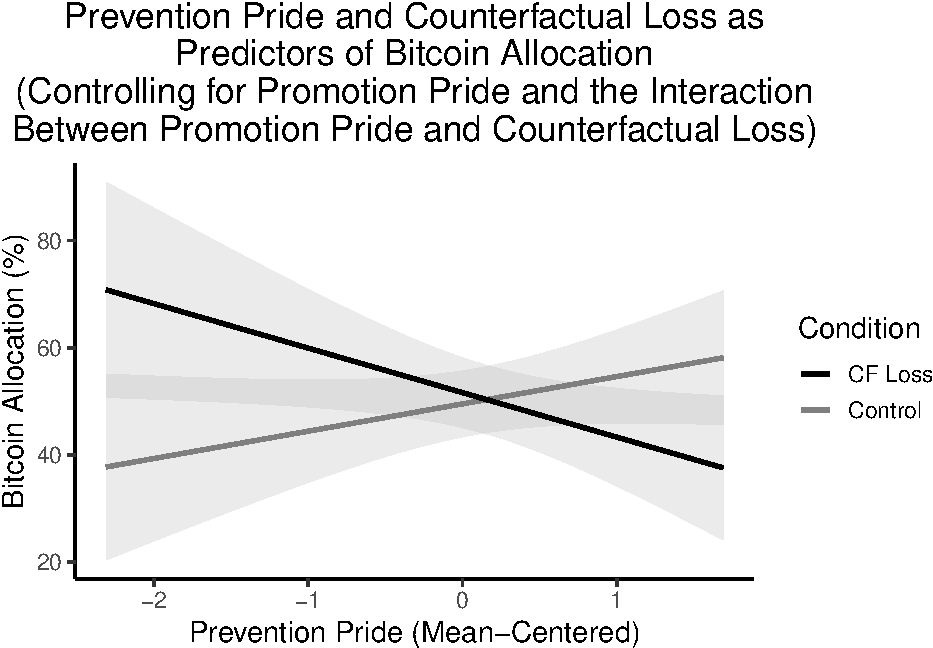
\includegraphics[width=0.9\linewidth,height=0.9\textheight]{rfcfloss_manuscript_files/figure-latex/primarymodelplot-1} 

}

\caption{Predicted Bitcoin allocation by prevention pride and counterfactual loss experience controlling for promotion pride and the interaction between promotion pride and counterfactual loss. Error bars represent 95\% confidence intervals.}\label{fig:primarymodelplot}
\end{figure}

The results revealed no main effects, and the interaction between \emph{promotion} pride and counterfactual loss was not significant. However, the analysis yielded a significant two-way interaction between \emph{prevention} pride and counterfactual loss (and this interaction effect remained significant when analyzed including participants who learned about the study from other participants: \(B = -12.77, p < .05\)).\footnote{This interaction also remained significant when controlling for a range of demographic variables including gender (\(B = -13.68, p < .01\)), age (\(B = -13.03, p < .05\)), ethnicity (\(B = -12.97, p < .05\)), income (\(B = -13.32, p < .05\)), and education (\(B = -13.53, p < .05\))), as well as when \emph{not} including promotion pride as a covariate (\(B = -12.61, p < .05\)).} To probe the conditional effect of prevention pride at each level of the counterfactual loss variable, we conducted a simple slopes analysis using the R-package \emph{interactions} (Version 1.1.1; Long, 2019). The effect of prevention pride on Bitcoin allocation was significant in the counterfactual loss condition (\(B = -8.31, SE = 3.92, t = -2.12, p < .05\); 95\% CI {[}-16.0311, -0.5906{]}) but non-significant in the control condition. These results indicate that, when facing counterfactual loss, as prevention pride increased, participants allocated less to a risky Bitcoin investment.

Additionally, to explore the interaction at different levels of prevention pride (\(M = 3.44; SD = 0.89\)), we applied the Johnson--Neyman (J--N) technique using using the R-package \emph{interactions} (Version 1.1.1; Long, 2019). This analysis revealed that the conditional effect of counterfactual loss on Bitcoin allocation was \emph{positive} for people with prevention pride of less than 2.51 (\(B = 13.11, SE = 6.66, t = 1.97, p < .05\)), and \emph{negative} for people with prevention pride of greater than 4.57 (\(B = -14.55, SE = 7.39, t = -1.97, p < .05\)). These results suggest that individuals high versus low in prevention pride responded to counterfactual loss in different ways, while people with middling levels of prevention pride did not respond to counterfactual loss.

\hypertarget{exploratory-moderated-mediation-analysis}{%
\subsection{3.2. Exploratory Moderated Mediation Analysis}\label{exploratory-moderated-mediation-analysis}}

By treating our counterfactual thought and hypothetical emotion measures as alternative mediators of the interaction of interest, we explored potential mechanisms underlying the effect. To do so, we conducted path analyses using the R-package \emph{lavaan} (Version 0.6.3; Rosseel, 2012). First, all variables were standardized to facilitate effect size comparisons across models. Then, within each analysis, we specified two regression models and formulas for the conditional indirect, direct, and total effects of interest in accordance with recommended practice for moderated mediation (Preacher, Rucker, \& Hayes, 2007) and Model 8 within Hayes' PROCESS macro (2018). In the first model, we regressed the potential mediator on prevention pride, counterfactual loss, and the interaction between prevention pride and counterfactual loss, while also controlling for promotion pride and the interaction between promotion pride and counterfactual loss. In the second model, we regressed our dependent variable (Bitcoin allocation) on the same predictor variables plus the potential mediator of interest. Within these models, standard errors and confidence intervals were estimated using bootstrap methods.

Across the potential mediators tested, one was significant: the degree to which participants reported they would hypothetically have been relieved if they had invested in Bitcoin earlier. Table 2 contains the results of this analysis.\footnote{The results of all other exploratory mediation analyses can be found within the Supplementary Materials.}

\begin{table}

\caption{\label{tab:medmodel}Summary of Mediation Analysis}
\centering
\resizebox{\linewidth}{!}{
\begin{threeparttable}
\begin{tabular}[t]{lllllll}
\toprule
\multicolumn{1}{c}{Predictor} & \multicolumn{1}{c}{Estimate} & \multicolumn{1}{c}{SE} & \multicolumn{1}{c}{z} & \multicolumn{1}{c}{p} & \multicolumn{1}{c}{CI.lower} & \multicolumn{1}{c}{CI.upper}\\
\midrule
\addlinespace[0.3em]
\multicolumn{7}{l}{\textbf{Model 1 (DV = Hypothetical Relief)}}\\
\hspace{1em}Intercept & \multicolumn{1}{r}{-0.16} & \multicolumn{1}{r}{0.06} & \multicolumn{1}{r}{-2.58} & \multicolumn{1}{r}{0.010} & \multicolumn{1}{r}{-0.2793} & \multicolumn{1}{r}{-0.0383}\\
\hspace{1em}Prevention Pride & \multicolumn{1}{r}{-0.07} & \multicolumn{1}{r}{0.06} & \multicolumn{1}{r}{-1.20} & \multicolumn{1}{r}{0.232} & \multicolumn{1}{r}{-0.1819} & \multicolumn{1}{r}{0.0469}\\
\hspace{1em}Counterfactual Loss & \multicolumn{1}{r}{-0.07} & \multicolumn{1}{r}{0.06} & \multicolumn{1}{r}{-1.05} & \multicolumn{1}{r}{0.293} & \multicolumn{1}{r}{-0.1843} & \multicolumn{1}{r}{0.0614}\\
\hspace{1em}Prev. Pride x CF Loss & \multicolumn{1}{r}{-0.13} & \multicolumn{1}{r}{0.06} & \multicolumn{1}{r}{-2.28} & \multicolumn{1}{r}{0.022} & \multicolumn{1}{r}{-0.2458} & \multicolumn{1}{r}{-0.0162}\\
\hspace{1em}Promotion Pride & \multicolumn{1}{r}{-0.11} & \multicolumn{1}{r}{0.06} & \multicolumn{1}{r}{-1.85} & \multicolumn{1}{r}{0.064} & \multicolumn{1}{r}{-0.2282} & \multicolumn{1}{r}{0.0084}\\
\hspace{1em}Prom. Pride x CF Loss & \multicolumn{1}{r}{0.02} & \multicolumn{1}{r}{0.06} & \multicolumn{1}{r}{0.29} & \multicolumn{1}{r}{0.772} & \multicolumn{1}{r}{-0.1007} & \multicolumn{1}{r}{0.1371}\\
\addlinespace[0.3em]
\multicolumn{7}{l}{\textbf{Model 2 (DV = Bitcoin Allocation)}}\\
\hspace{1em}Intercept & \multicolumn{1}{r}{0.06} & \multicolumn{1}{r}{0.06} & \multicolumn{1}{r}{0.97} & \multicolumn{1}{r}{0.334} & \multicolumn{1}{r}{-0.0654} & \multicolumn{1}{r}{0.1812}\\
\hspace{1em}Prevention Pride & \multicolumn{1}{r}{0.02} & \multicolumn{1}{r}{0.06} & \multicolumn{1}{r}{0.28} & \multicolumn{1}{r}{0.782} & \multicolumn{1}{r}{-0.0973} & \multicolumn{1}{r}{0.1416}\\
\hspace{1em}Counterfactual Loss & \multicolumn{1}{r}{0.04} & \multicolumn{1}{r}{0.06} & \multicolumn{1}{r}{0.64} & \multicolumn{1}{r}{0.523} & \multicolumn{1}{r}{-0.0825} & \multicolumn{1}{r}{0.1654}\\
\hspace{1em}Prev. Pride x CF Loss & \multicolumn{1}{r}{-0.08} & \multicolumn{1}{r}{0.06} & \multicolumn{1}{r}{-1.41} & \multicolumn{1}{r}{0.160} & \multicolumn{1}{r}{-0.2031} & \multicolumn{1}{r}{0.0368}\\
\hspace{1em}Promotion Pride & \multicolumn{1}{r}{0.15} & \multicolumn{1}{r}{0.06} & \multicolumn{1}{r}{2.36} & \multicolumn{1}{r}{0.018} & \multicolumn{1}{r}{0.0285} & \multicolumn{1}{r}{0.2761}\\
\hspace{1em}Prom. Pride x CF Loss & \multicolumn{1}{r}{0.06} & \multicolumn{1}{r}{0.06} & \multicolumn{1}{r}{0.92} & \multicolumn{1}{r}{0.356} & \multicolumn{1}{r}{-0.0654} & \multicolumn{1}{r}{0.1783}\\
\hspace{1em}Hypothetical Relief & \multicolumn{1}{r}{0.42} & \multicolumn{1}{r}{0.07} & \multicolumn{1}{r}{6.44} & \multicolumn{1}{r}{< .001} & \multicolumn{1}{r}{0.2888} & \multicolumn{1}{r}{0.5510}\\
\addlinespace[0.3em]
\multicolumn{7}{l}{\textbf{\makecell[l]{Bootstrapped Conditional Indirect Effects\\(Prev. Pride x CF Loss → Hypothetical Relief → Bitcoin Allocation)}}}\\
\hspace{1em}Control Condition & \multicolumn{1}{r}{0.03} & \multicolumn{1}{r}{0.03} & \multicolumn{1}{r}{0.77} & \multicolumn{1}{r}{0.440} & \multicolumn{1}{r}{-0.0421} & \multicolumn{1}{r}{0.0923}\\
\hspace{1em}Counterfactual Loss Condition & \multicolumn{1}{r}{-0.09} & \multicolumn{1}{r}{0.04} & \multicolumn{1}{r}{-2.30} & \multicolumn{1}{r}{0.021} & \multicolumn{1}{r}{-0.1614} & \multicolumn{1}{r}{-0.0141}\\
\bottomrule
\end{tabular}
\begin{tablenotes}[para]
\item \textit{Note: } 
\item This analysis included an effect-coded variable for the counterfactual loss condition: -1 = control, 1 = counterfactual loss. All other variables were standardized (M = 0, SD = 1). Estimated effect sizes for the models reported here are standardized regression coefficients.
\end{tablenotes}
\end{threeparttable}}
\end{table}

The interaction between prevention pride and counterfactual loss was associated with hypothetical relief (\(\beta = -0.13\), \(p < .05\)), and the effect of hypothetical relief was associated with Bitcoin allocation (\(\beta = 0.42\), \(p < .001\)). Importantly, the indirect effect of prevention pride on Bitcoin allocation through hypothetical relief was significant and negative for individuals in the counterfactual loss condition (\(\beta = -0.09\), \(SE = 0.04\), 95\% CI {[}\(-0.1614, -0.0141\){]}), but not the control condition (n.s.). This finding indicates that the moderation is fully mediated.

\hypertarget{discussion}{%
\section{4. Discussion}\label{discussion}}

Regulatory focus has been well-established as an individual difference that predicts unique patterns of decision-making. The purpose of the present study was to examine whether the effect of a prevention focus on risky choices following actual loss (Scholer et al., 2010) translates to cases of socially-defined counterfactual loss.

The results of our primary analysis indicated that a prevention focus does indeed predict the degree to which participants engage in risk-taking following a socially-defined counterfactual loss. These findings suggest that counterfactual loss is uniquely relevant to the prevention (vs.~promotion) system. Our exploratory mediation analysis provides further support for this relationship, as the hypothetical emotional experience that mediates the interaction effect (i.e., hypothetical relief) falls on the quiescence-agitation spectrum that relates to prevention.

However, the direction of this effect contradicted our primary hypothesis: Although we hypothesized that a prevention focus would predict increased risk-taking in cases of counterfactual loss, we found that prevention pride predicted \emph{decreased} risky investment behavior in such a case. Interestingly, these findings \emph{do} align with the alternate account introduced in section 1.1.

\hypertarget{limitations-and-future-research}{%
\subsection{4.1. Limitations and Future Research}\label{limitations-and-future-research}}

Despite its contributions, this study had several limitations. First, the study was intended to place participants in a situation in which the only way to recover a counterfactually-lost amount would be to make a risky investment. However, our findings suggest that participants may not have believed that investing in Bitcoin offered them this opportunity for full recovery. To guarantee that the risky option offers this possibility, a replication study might allow participants to participate in a game of chance that explicitly provides the opportunity to earn this amount. For example, upon learning that they would join the beta-test on Day 4, participants could be offered the opportunity to pay a small amount to spin a wheel with a chance of winning the \enquote{lost} \$0.61.

A second limitation is that our predictions were rooted in the assumption that the experience of counterfactual loss is created by the introduction of a social reference point above one's current status quo, which then redefines what constitutes a satisfactory state. However, the study did not examine this change in reference points explicitly, and follow-up studies should do so. For instance, at the start of the study, participants could be asked to consider their financial goal pursuits and then visualize their current status quo and what they would consider a satisfactory state as points on a line. Later, following the counterfactual loss manipulation, participants might repeat this procedure. We predict that the point representing the current state would not shift, while the point representing the satisfactory state would increase in distance with respect to the current state---particularly for prevention-focused participants.

Finally, future studies should also examine the impact of regulatory focus in other counterfactual situations. In particular, given Zou and colleagues' (2014) finding that a promotion focus predicts risky decision-making in cases of actual gains, the results of the present study suggest that a consistent effect may be present in cases of counterfactual gains.

\hypertarget{implications-and-conclusions}{%
\subsection{4.2 Implications and Conclusions}\label{implications-and-conclusions}}

The present research offers several important implications. First, it contributes to the regulatory focus literature by extending Scholer and colleagues' (2010) findings to the domain of counterfactual loss. Additionally, the research raises the intriguing question of whether the reference point one considers a satisfactory status-quo may dynamically shift as a function of the social context.

Finally, this research has important ramifications for individuals making financial decisions. For instance, consider the real estate market; if friends purchase a home that appreciates during a housing \enquote{bubble,} individual differences like regulatory focus may affect a person's propensity to riskily invest in an overvalued home. Given these real-world implications, follow-up studies should investigate how people with a prevention focus can manage these tendencies that may ultimately detract from their well-being.

\newpage

\hypertarget{references}{%
\section{References}\label{references}}

\begingroup
\setlength{\parindent}{-0.5in}
\setlength{\leftskip}{0.5in}

\hypertarget{refs}{}
\leavevmode\hypertarget{ref-bonezzietal2011}{}%
Bonezzi, A., Brendl, C. M., \& De Angelis, M. (2011). Stuck in the middle: The psychophysics of goal pursuit. \emph{Psychological Science}, \emph{22}(5), 607--612. \url{https://doi.org/10.1177/0956797611404899}

\leavevmode\hypertarget{ref-R-shiny}{}%
Chang, W., Cheng, J., Allaire, J., Xie, Y., \& McPherson, J. (2018). \emph{Shiny: Web application framework for r}. Retrieved from \url{https://CRAN.R-project.org/package=shiny}

\leavevmode\hypertarget{ref-hayes2018}{}%
Hayes, A. F. (2018). \emph{Introduction to mediation, moderation, and conditional process analysis: A regression-based approach}. (D. A. Kenny \& T. D. Little, Eds.) (2nd ed.). New York, NY: The Guildford Press.

\leavevmode\hypertarget{ref-heathetal1999}{}%
Heath, C., Larrick, R. P., \& Wu, G. (1999). Goals as reference points. \emph{Cognitive Psychology}, \emph{38}(1), 79--109. \url{https://doi.org/10.1006/cogp.1998.0708}

\leavevmode\hypertarget{ref-higgins1996d}{}%
Higgins, E. T. (1996). Emotional experiences: The pains and pleasures of distinct regulatory systems. In R. D. Kavanaugh, B. Zimmerberg, \& S. Fein (Eds.), \emph{Emotion: Interdisciplinary perspectives} (pp. 203--241). Mahwah, NJ: Lawrence Erlbaum Associates. Retrieved from \url{https://books.google.com/books?id=iok2pKzHAfQC\&printsec=frontcover\&source=gbs_ViewAPI\#v=onepage\&q\&f=false}

\leavevmode\hypertarget{ref-higgins1997}{}%
Higgins, E. T. (1997). Beyond pleasure and pain. \emph{American Psychologist}, \emph{52}(12), 1280--1300. \url{https://doi.org/10.1037/0003-066X.52.12.1280}

\leavevmode\hypertarget{ref-higgins2018}{}%
Higgins, E. T. (2018). What distinguishes promotion and prevention? Attaining ``+1'' from ``0'' as non-gain versus maintaining ``0'' as non-loss. \emph{Polish Psychological Bulletin}, \emph{49}(1), 40--49. \url{https://doi.org/10.24425/119470}

\leavevmode\hypertarget{ref-higginscornwell2016}{}%
Higgins, E. T., \& Cornwell, J. F. M. (2016). Securing foundations and advancing frontiers: Prevention and promotion effects on judgment \& decision making. \emph{Organizational Behavior and Human Decision Processes}, \emph{136}, 56--67. \url{https://doi.org/10.1016/j.obhdp.2016.04.005}

\leavevmode\hypertarget{ref-higginsetal2001}{}%
Higgins, E. T., Friedman, R., Harlow, R. E., Idson, L. C., Ayduk, O. N., \& Taylor, A. (2001). Achievement orientations from subjective histories of success: Promotion pride versus prevention pride. \emph{European Journal of Social Psychology}, \emph{31}(1), 3--23. \url{https://doi.org/10.1002/ejsp.27}

\leavevmode\hypertarget{ref-higginsliberman2018}{}%
Higgins, E. T., \& Liberman, N. (2018). The loss of loss aversion: Paying attention to reference points. \emph{Journal of Consumer Psychology}, \emph{28}(3), 523--532. \url{https://doi.org/10.1002/jcpy.1045}

\leavevmode\hypertarget{ref-higginsetal1997}{}%
Higgins, E. T., Shah, J., \& Friedman, R. (1997). Emotional responses to goal attainment: Strength of regulatory focus as moderator. \emph{Journal of Personality and Social Psychology}, \emph{72}(3), 515--525. \url{https://doi.org/10.1037/0022-3514.72.3.515}

\leavevmode\hypertarget{ref-higginsetal1986a}{}%
Higgins, E. T., Strauman, T., \& Klein, R. (1986). Standards and the process of self-evaluation: Multiple affects from multiple stages. In R. M. Sorrentino \& E. T. Higgins (Eds.), \emph{Handbook of motivation and cognition: Foundations of social behavior} (pp. 435--464). New York, NY: Guilford Press.

\leavevmode\hypertarget{ref-inmanzeelenberg2002}{}%
Inman, J. J., \& Zeelenberg, M. (2002). Regret in repeat purchase versus switching decisions: The attenuating role of decision justifiability. \emph{Journal of Consumer Research}, \emph{29}(1), 116--128. \url{https://doi.org/10.1086/339925}

\leavevmode\hypertarget{ref-kennedyetal2018}{}%
Kennedy, R., Clifford, S., Burleigh, T., Jewell, R., \& Waggoner, P. (2018). \emph{The shape of and solutions to the MTurk quality crisis} (SSRN Scholarly Paper No. ID 3272468). Rochester, NY: Social Science Research Network. Retrieved from \url{https://papers.ssrn.com/abstract=3272468}

\leavevmode\hypertarget{ref-R-rIP}{}%
Kennedy, R., \& Waggoner, P. (2018). \emph{RIP: Detects fraud in online surveys by tracing and scoring ip addresses}. Retrieved from \url{https://CRAN.R-project.org/package=rIP}

\leavevmode\hypertarget{ref-kruglanskietal2000}{}%
Kruglanski, A. W., Thompson, E. P., Higgins, E. T., Atash, M. N., Pierro, A., Shah, J. Y., \& Spiegel, S. (2000). To "do the right thing" or to "just do it": Locomotion and assessment as distinct self-regulatory imperatives. \emph{Journal of Personality and Social Psychology}, \emph{79}(5), 793--815. \url{https://doi.org/10.1037/0022-3514.79.5.793}

\leavevmode\hypertarget{ref-R-interactions}{}%
Long, J. A. (2019). \emph{Interactions: Comprehensive, user-friendly toolkit for probing interactions}. Retrieved from \url{https://cran.r-project.org/package=interactions}

\leavevmode\hypertarget{ref-preacheretal2007}{}%
Preacher, K. J., Rucker, D. D., \& Hayes, A. F. (2007). Addressing moderated mediation hypotheses: Theory, methods, and prescriptions. \emph{Multivariate Behavioral Research}, \emph{42}(1), 185--227. \url{https://doi.org/10.1080/00273170701341316}

\leavevmode\hypertarget{ref-R-base}{}%
R Core Team. (2018). \emph{R: A language and environment for statistical computing}. Vienna, Austria: R Foundation for Statistical Computing. Retrieved from \url{https://www.R-project.org/}

\leavevmode\hypertarget{ref-R-lavaan}{}%
Rosseel, Y. (2012). lavaan: An R package for structural equation modeling. \emph{Journal of Statistical Software}, \emph{48}(2), 1--36. Retrieved from \url{http://www.jstatsoft.org/v48/i02/}

\leavevmode\hypertarget{ref-scholeretal2010}{}%
Scholer, A. A., Zou, X., Fujita, K., Stroessner, S. J., \& Higgins, E. T. (2010). When risk seeking becomes a motivational necessity. \emph{Journal of Personality and Social Psychology}, \emph{99}(2), 215--231. \url{https://doi.org/10.1037/a0019715}

\leavevmode\hypertarget{ref-zouscholer2016}{}%
Zou, X., \& Scholer, A. A. (2016). Motivational affordance and risk-taking across decision domains. \emph{Personality and Social Psychology Bulletin}, \emph{42}(3), 275--289. \url{https://doi.org/10.1177/0146167215626706}

\leavevmode\hypertarget{ref-zouetal2014}{}%
Zou, X., Scholer, A. A., \& Higgins, E. T. (2014). In pursuit of progress: Promotion motivation and risk preference in the domain of gains. \emph{Journal of Personality and Social Psychology}, \emph{106}(2), 183--201. \url{https://doi.org/10.1037/a0035391}

\endgroup


\end{document}
